\documentclass[12pt, oneside]{article}   	% use "amsart" instead of "article" for AMSLaTeX format

\usepackage{graphicx}
\graphicspath{ {\string} }
\usepackage{subcaption}

%%%%%%%%%%%%%%%%%%%%%%%%%%%%%%%%%%%%%%%%%%%%%%%%%%%%
% set up packages
%%%%%%%%%%%%%%%%%%%%%%%%%%%%%%%%%%%%%%%%%%%%%%%%%%%%
\usepackage{geometry}                
\usepackage{textcomp}                
\usepackage{amsmath}                
\usepackage{graphicx}                
\usepackage{amssymb}                
\usepackage{fancyhdr}                
\usepackage{subcaption}                
\usepackage{bm}                
\usepackage{lineno}
% package for comments
\usepackage{soul}     
\usepackage{setspace}

\usepackage{mathtools}
\usepackage{physics}
\usepackage{xcolor}

\usepackage{tikz}
\usetikzlibrary{decorations.pathreplacing,positioning, arrows.meta}
%%%%%%%%%%%%%%%%%%%%%%%%%%%%%%%%%%%%%%%%%%%%%%%%%%%%
% call packages
%%%%%%%%%%%%%%%%%%%%%%%%%%%%%%%%%%%%%%%%%%%%%%%%%%%%	
\geometry{letterpaper, marginparwidth=60pt} % sets up geometry              		
\linenumbers % adds line numbers 
%\doublespacing % setspace
	
\usepackage[superscript,noadjust]{cite} % puts dash in citations to abbreviate
%\usepackage [autostyle, english = american]{csquotes} % sets US-style quotes
%\MakeOuterQuote{"} % sets quote style

\usepackage{hyperref}
\hypersetup{
    colorlinks=true,
    linkcolor=blue,
    filecolor=magenta,      
    urlcolor=cyan,
}

\usepackage{tabularx}

\usepackage{etoolbox}
\AtBeginEnvironment{quote}{\small}

\usepackage{float,color}
\usepackage{xcolor}
\definecolor{darkspringgreen}{rgb}{0.09, 0.45, 0.27}

\usepackage[section]{placeins}

\usepackage{tikz-qtree}
\usetikzlibrary{trees}

\usepackage{natbib}
%\bibliographystyle{abbrvnat}
\setcitestyle{authoryear,open={(},close={)}}

%%%%%%%%%%%%%%%%%%%%%%%%%%%%%%%%%%%%%%%%%%%%%%%%%%%%

%%%%%%%%%%%%%%%%%%%%%%%%%%%%%%%%%%%%%%%%%%%%%%%%%%%%
\pagestyle{plain}                                                      %%
%%%%%%%%%% EXAFT 1in MARGINS %%%%%%%                                   %%
\setlength{\textwidth}{6.5in}     %%                                   %%
\setlength{\oddsidemargin}{0in}   %% (It is recommended that you       %%
\setlength{\evensidemargin}{0in}  %%  not change these parameters,     %%
\setlength{\textheight}{8.5in}    %%  at the risk of having your       %%
\setlength{\topmargin}{0in}       %%  proposal dismissed on the basis  %%
\setlength{\headheight}{0in}      %%  of incorrect formatting!!!)      %%
\setlength{\headsep}{0in}         %%                                   %%
\setlength{\footskip}{.5in}       %%                                   %%
%%%%%%%%%%%%%%%%%%%%%%%%%%%%%%%%%%%%                                   %%		

%%%%%%%%%%%%%
% DEFINE CODE BLOCK
%%%%%%%%%%%%%
\usepackage{listings}

\definecolor{dkgreen}{rgb}{0,0.6,0}
\definecolor{gray}{rgb}{0.5,0.5,0.5}
\definecolor{mauve}{rgb}{0.58,0,0.82}

\lstset{frame=tb,
  language=R,
  aboveskip=3mm,
  belowskip=3mm,
  showstringspaces=false,
  columns=flexible,
  basicstyle={\small\ttfamily},
  numbers=none,
  numberstyle=\tiny\color{gray},
 % keywordstyle=\color{blue},
  commentstyle=\color{dkgreen},
  stringstyle=\color{mauve},
  breaklines=true,
  breakatwhitespace=true,
  tabsize=3,
  otherkeywords={0,1,2,3,4,5,6,7,8,9},
  deletekeywords={data,frame,length,as,character,dunif,ps},
}

%%%%%%%%%%%%%%%%%%%%%%%%%%%%%%%%%%%%%%%%%%%%%%%%%%%%
\usepackage{tikz}
\usetikzlibrary{arrows,automata}
\usetikzlibrary{positioning}


%%%%%%%%%%%%%%%%%%%%%%%%%%%%%%%%%%%%%%%%%%%%%%%%%%%%

\begin{document} 

\section*{Unbranched plant with a terminal, determinate flower}

The case we consider here is the one for a plant that does not branch and has a terminal, determinate flower. The unbranched, vegetative architecture is established by primary meristem divisions that generate a vegetative meristem and leaf (\hl{Figure 1A}); because there is never more than one vegetative meristem, the plant does not branch. At the transition to flowering, the vegetative meristem transitions to an inflorescence meristem (\hl{Figure 1B}). Finally, the terminal, determinate flower is represented in the model by the transition from the inflorescence meristem to a flower (\hl{Figure 1C}).

\begin{figure}[hbt!]
%% PRIMARY MERISTEM PRODUCING PRIMARY MERISTEM
  \begin{subfigure}{.25\textwidth}
  \centering
    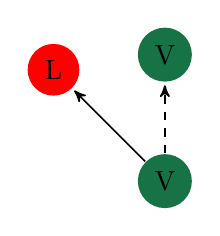
\begin{tikzpicture}[->,>=stealth',shorten >=1pt,auto,node distance=2cm,semithick]
  \tikzstyle{every state}=[draw=none]

  \node[state, fill=darkspringgreen,minimum size=.5cm] 	     (A)                    {V};
  \node[state, fill=red,minimum size=.5cm]         (B) [above left of=A] {L};
  \node[state, fill=darkspringgreen,minimum size=.5cm] 	     (D) [above =.9cm of A]                   {V};

  \path[dashed] (A) edge              (D);
  \path[->] (A) edge (B);

      \end{tikzpicture}
          \caption{Vegetative meristem transitioning to one vegetative meristem and generating one leaf.} 
  \end{subfigure}
              \hspace{\fill}
%% PRIMARY MERISTEM PRODUCING INFLORESCENCE MERISTEM
\begin{subfigure}{.25\textwidth}
    \centering
      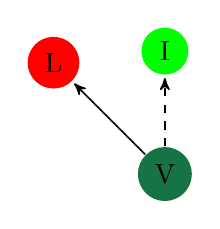
\begin{tikzpicture}[->,>=stealth',shorten >=1pt,auto,node distance=2cm,
                    semithick,text=black]

  \node[state, fill = darkspringgreen, draw = none,minimum size=.5cm] (A)                    {V};
  \node[state, fill = red, draw = none,minimum size=.5cm]         (B) [above left of=A] {L};
  \node[state, fill=green, draw = none,minimum size=.5cm] 	     (C) [above =.9cm of A]                   {I};

  \path[dashed] (A) edge              (C);
  \path[->] (A) edge (B);

      \end{tikzpicture}
    \caption{Vegetatuve meristem transitioning to one vegetative meristem, and generating one inflorescence meristem.}
      \end{subfigure}
          \hspace{\fill}
%% PRIMARY MERISTEM PRODUCING INFLORESCENCE MERISTEM
      \begin{subfigure}{.25\textwidth}
\centering
      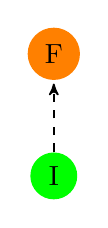
\begin{tikzpicture}[->,>=stealth',shorten >=1pt,auto,node distance=2cm,
                    semithick,text=black]

  \node[state, fill = green, draw = none,minimum size=.5cm] (A)                    {I};
  \node[state, fill = orange, draw = none,minimum size=.5cm]         (B) [above =.9cm of A] {F};
  \path[dashed] (A) edge              (B);

      \end{tikzpicture}
    \caption{Inflorescence meristem generating a flower.}
  \end{subfigure}
        \caption{State variable transitions in an unbranched plant with a terminal, determinate flower.}
    \label{fig:transitions-unbranched-determinate}
\end{figure}

The table below summarizes the state and control variables in the model.

\singlespace
\begin{table}[hbt!]
\footnotesize
\begin{tabularx}{\linewidth}{l X l}
\hline
 \hline
\multicolumn{1}{ l }{ Symbol } & 
\multicolumn{1}{ c }{ Description } &
\multicolumn{1}{ c }{ Units } \\

\hline
\multicolumn{3}{ l }{ \sc{State variables }} \\
 $V(t)$   & Vegetative meristem population size & number of vegetative meristems \\ 
 $L(t)$   & Leaf population size & number of leaves \\ 
 $I(t)$   & Inflorescence meristem population size & number of inflorescence meristems \\ 
 $F(t)$   & Flower population size & number of flowers \\ 
\hline

\end{tabularx}
\end{table}
%\doublespace

\clearpage
\newpage

In this case, there is 1 vegetative meristem that transitions to 1 inflorescence meristem at the transition to flowering. Because there there is only 1 vegetative meristem, there is a single transition to flowering (the solution is bang-bang) at the switch time $\theta$. Before the transition to flowering, the plant accumulates leaf biomass; after the transition to flowering there is no additional accumulation of leaf biomass. At the transition to flowering, the plant has accumulated L($\theta$) leaves, which then remains constant to the end of the season. With a terminal, determinate flower, the plant can develop at most 1 flower. The figure below illustrates the assumptions described here:

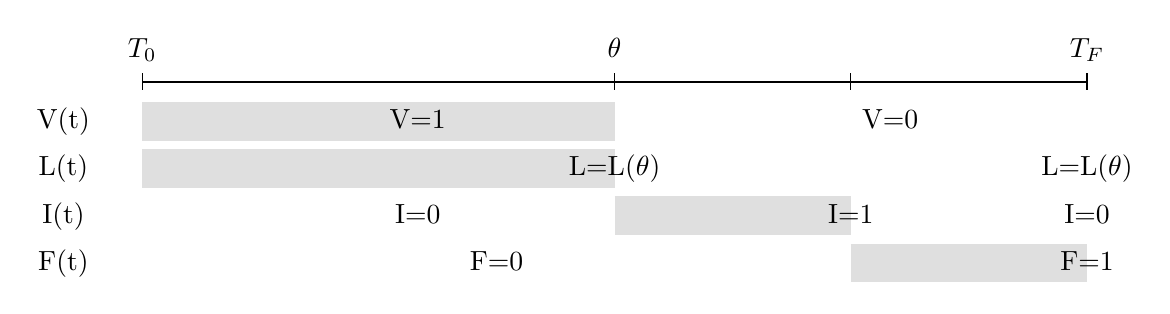
\begin{tikzpicture}

% draw horizontal line   
\draw[thick] (0,0) -- (12,0) node[font=\normalsize,below left=3pt and -8pt]{};

% draw vertical lines
\foreach \x in {0,6,9,12}
\draw (\x cm,3pt) -- (\x cm,-3pt);

% dates
\foreach \x/\descr in {0/$T_0$,{6}/$\theta$,{9}/$$,{12}/$T_F$}
\node[font=\normalsize, text height=1.75ex, text depth=.5ex] at (\x,.4) {{\descr}};

% ROUND 1
% Age 1
\foreach \x/\perccol in
{0/50,1/50,2/50,3/50,4/50,5/50}
\draw[lightgray!\perccol!white, line width=14pt] 
(\x,-.5) -- +(1,0);

% Age 2
\foreach \x/\perccol in
{0/50,1/50,2/50,3/50,4/50,5/50}
\draw[lightgray!\perccol!white, line width=14pt] 
(\x,-1.1) -- +(1,0);

% Age 3
\foreach \x/\perccol in
{6/50,7/50,8/50}
\draw[lightgray!\perccol!white, line width=14pt] 
(\x,-1.7) -- +(1,0);

% Age 4
\foreach \x/\perccol in
{9/50,10/50,11/50}
\draw[lightgray!\perccol!white, line width=14pt] 
(\x,-2.3) -- +(1,0);

\node [font=\normalsize, text height=1.75ex, text depth=.5ex] at (-1,-.5) {V(t)};
\node [font=\normalsize, text height=1.75ex, text depth=.5ex] at (3.5,-.5) {V=1};
\node [font=\normalsize, text height=1.75ex, text depth=.5ex] at (9.5,-.5) {V=0};

\node [font=\normalsize, text height=1.75ex, text depth=.5ex] at (-1,-1.1) {L(t)};
\node [font=\normalsize, text height=1.75ex, text depth=.5ex] at (6,-1.1) {L=L($\theta$)};
\node [font=\normalsize, text height=1.75ex, text depth=.5ex] at (12,-1.1) {L=L($\theta$)};

\node [font=\normalsize, text height=1.75ex, text depth=.5ex] at (-1,-1.7) {I(t)};
\node [font=\normalsize, text height=1.75ex, text depth=.5ex] at (3.5,-1.7) {I=0};
\node [font=\normalsize, text height=1.75ex, text depth=.5ex] at (9,-1.7) {I=1};
\node [font=\normalsize, text height=1.75ex, text depth=.5ex] at (12,-1.7) {I=0};

\node [font=\normalsize, text height=1.75ex, text depth=.5ex] at (-1,-2.3) {F(t)};
\node [font=\normalsize, text height=1.75ex, text depth=.5ex] at (4.5,-2.3) {F=0};
\node [font=\normalsize, text height=1.75ex, text depth=.5ex] at (12,-2.3) {F=1};
\end{tikzpicture}

The plant must make a flower before the end of the season, subject to resource constraints and constraints on meristem division rates. Because the solution is known to be bang-bang, the optimal strategy is the one that simultaneously minimizes the sum of the switch time ($\theta$; ensuring the onset of reproduction), the time to produce the inflorescence meristem ($\tau_1$), and the time to produce the flower ($\tau_2$). The optimization problem is then:
%
\begin{align}
\min_{\theta} & \ \theta + \tau_1 + \tau_2  \nonumber
\end{align}

The meristem division rates $M_0, M_1, M_2$ are the fixed, upper limits on the per-capita rates at which the divisions in \hl{Figure 1A-C} take place (units of meristems/(meristem time)). The conversion rate of standing biomass, $\alpha$, describes the energy produced by a unit of leaf.

\begin{align}
\dot{L} = \mathrm{min}(\alpha L(t), M_0) \nonumber \\
\tau_1 = \frac{1}{\mathrm{min}(M_1,\alpha L(\theta) )} \nonumber \\ 
\tau_2 = \frac{1}{\mathrm{min}(M_2,\alpha L(\theta) )} \nonumber
\end{align}

For each combination of $M_0, M_1, M_2, \alpha$, the objective function can be calculated by:

\begin{itemize}
\item Solve $\dot{L} = \mathrm{min}(\alpha L(t), M_0)$ to the switch time $\theta$
\item Calculate $L(\theta)$
\item Use $L(\theta), M_1, M_2$ to calculate $\tau_1, \tau_2$
\item Calculate $\theta + \tau_1 + \tau_2  \nonumber$
\end{itemize}

The optimal switch time is the one that minimizes the last line in the algorithm above.

\subsubsection{Resource constraint only}
When $M_i$ approaches $\infty$ (case without meristem constraint), the problem becomes the following. 

\begin{align}
\dv{L}{t} = \alpha L \nonumber
\end{align}

\begin{align}
\int_{0}^{\theta} \dv{L}{t} =\int_{0}^{\theta} \alpha L \nonumber \\
\int_{0}^{\theta} \frac{\mathrm{d}L}{L} =\int_{0}^{\theta} \alpha \mathrm{d}t \nonumber \\
\log(L(\theta)) - \log(L(0)) = \alpha \theta - \alpha 0 \nonumber \\
\log(\frac{L(\theta)}{L(0)}) = \alpha \theta \nonumber \\
\frac{L(\theta)}{L(0)} = \exp^{\alpha \theta} \nonumber \\
L(\theta) = L(0) \exp^{\alpha \theta} \nonumber 
\end{align}

This means

\begin{align}
\tau_1 = \frac{1}{\alpha L(0) \exp^{\alpha \theta}} \nonumber \\ 
\tau_2 = \frac{1}{\alpha L(0) \exp^{\alpha \theta}} \nonumber
\end{align}

so the minimization is 

\begin{align}
\min_{\theta} & \ \theta + \frac{2}{\alpha L(0) \exp^{\alpha \theta}}  \nonumber
\end{align}

\clearpage
\newpage

\subsubsection{Meristem constraint only}
When $\alpha$ approaches $\infty$ (case without resource constraint), the problem becomes the following. 

\begin{align}
\dv{L}{t} = M_0
\end{align}

\begin{align}
\dot{L} =  M_0 \nonumber \\
\tau_1 = \frac{1}{M_1} \nonumber \\ 
\tau_2 = \frac{1}{M_2}. \nonumber
\end{align}

The plant should immediately transition to reproduction, $\theta=0$, which is completed according to

\begin{align}
\tau_1 + \tau_2 = \frac{1}{M_1} + \frac{1}{M_2}.  \nonumber
\end{align}

\clearpage
\newpage

\begin{figure}[!h]
       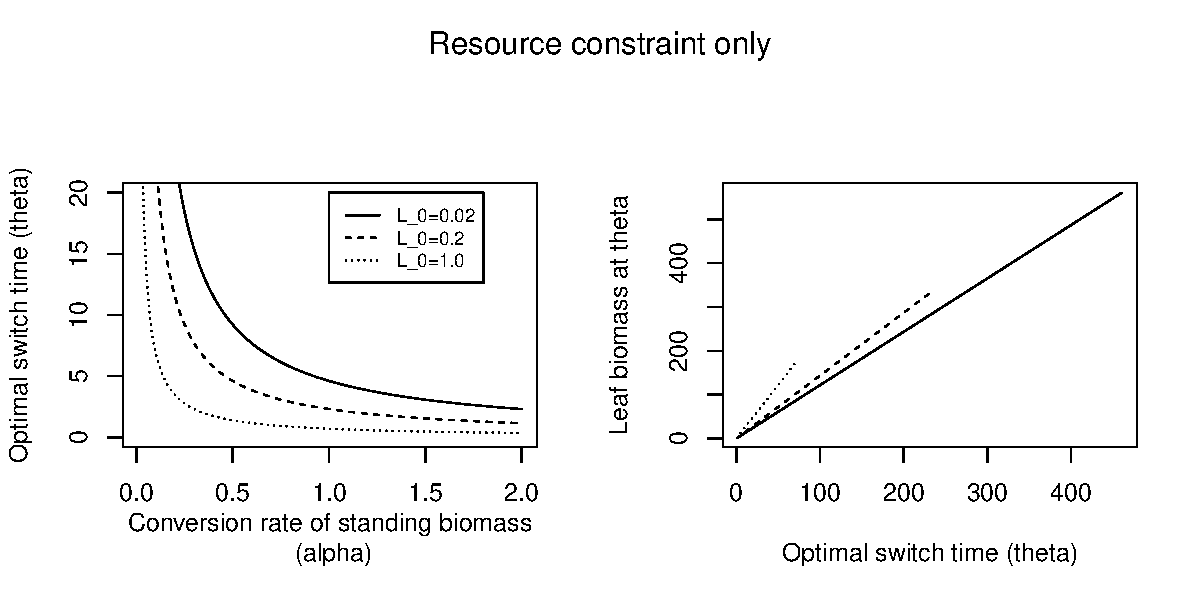
\includegraphics[width=\textwidth]{../../figures/1d-resource-only.pdf}  
    \caption{ Properties of the optimal switch time for a 1D, unbranched plant without a meristem constraint. (A) If all per-capita rates of meristem division approach infinity, the optimal switch time decreases as the conversion rate of standing biomass ($\alpha$) increases  for a given initial amount of leaf biomass $L_0$. (B) The optimal switch time $\theta$ is linearly related to the leaf biomass at the transition to flowering.   }
 \label{fig:figure-x}
\end{figure}


\clearpage
\newpage

\begin{figure}[!h]
       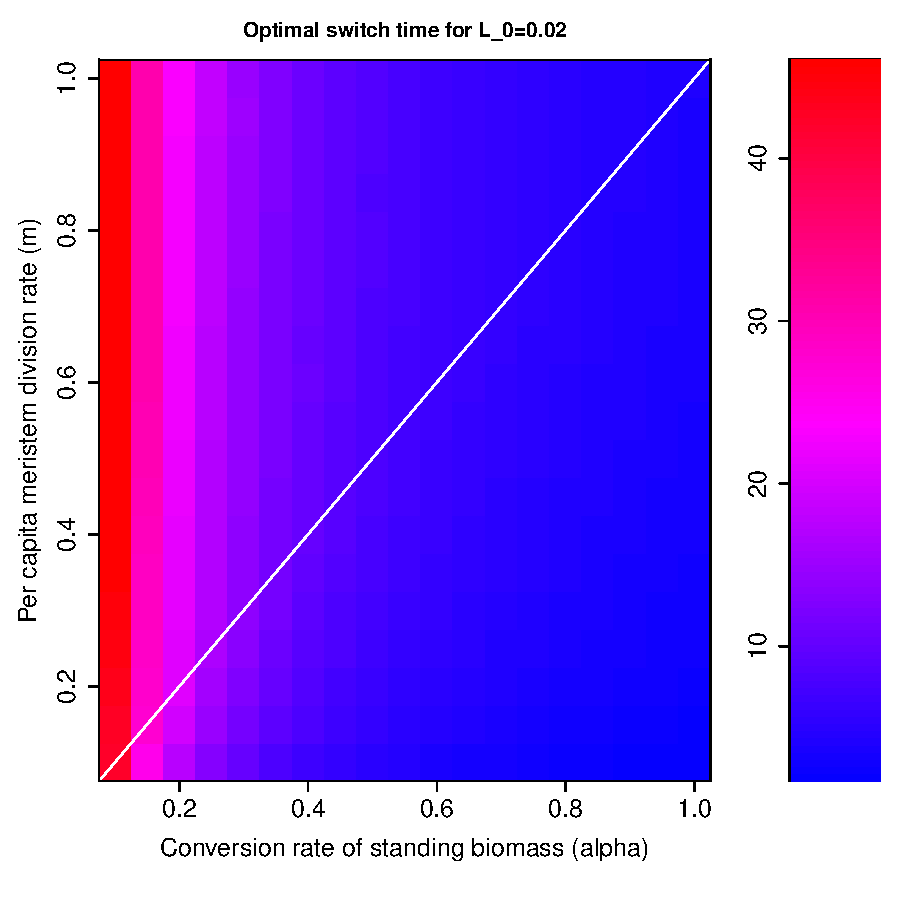
\includegraphics[width=.5\textwidth]{../../figures/1d-0.02-zoom.pdf}  
       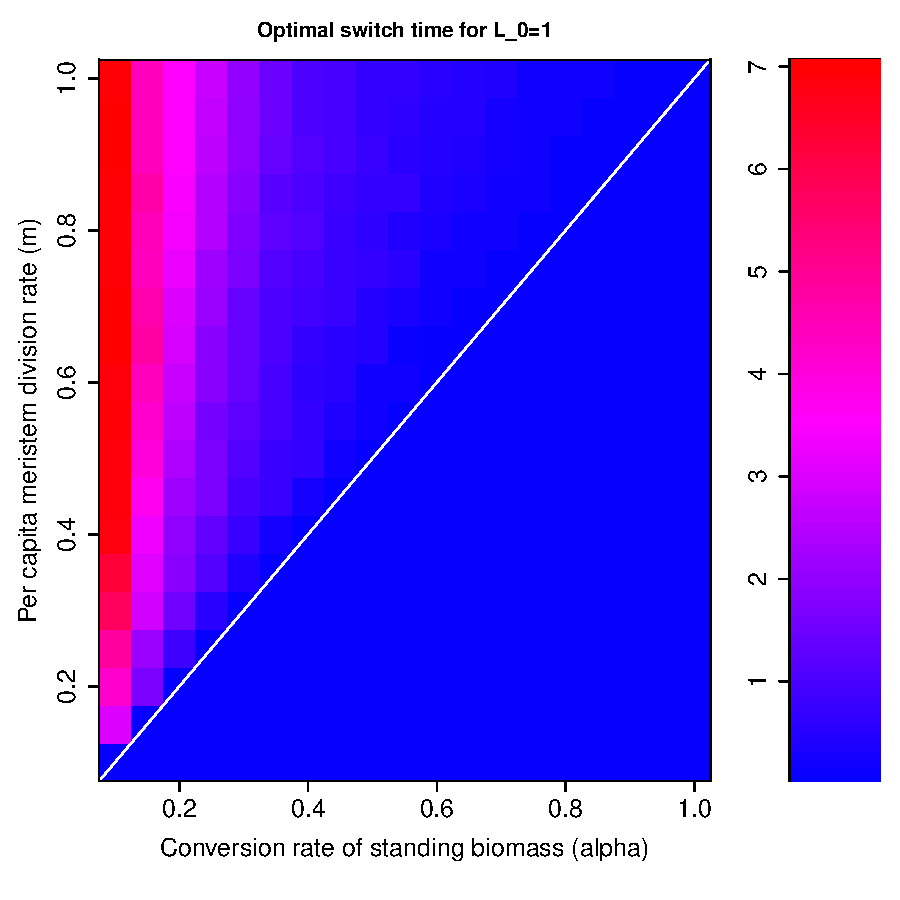
\includegraphics[width=.5\textwidth]{../../figures/1d-1-zoom.pdf}  
    \caption{ Properties of the optimal switch time for a 1D, unbranched plant. (A) Optimal switch time across a grid of $\alpha \times \mathrm{m}$ for initial leaf mass value of $L_0 = 0.02$. The range of switch times $\theta$ is from (0,40). (B) Optimal switch time across a grid of $\alpha \times \mathrm{m}$ for initial leaf mass value of $L_0 = 1$. The range of switch times $\theta$ is from (0,7).   }
 \label{fig:figure-x}
\end{figure}

\begin{figure}[!h]
       \includegraphics[width=.5\textwidth,page=2]{../../figures/1d-0.02-zoom.pdf}  
       \includegraphics[width=.5\textwidth,page=2]{../../figures/1d-1-zoom.pdf}  
    \caption{ Optimal switch time plotted against conversion rate of standing biomass. Lighter colors are low meristem division rates and darker colors are higher meristem division rates ($0\leq m \leq 1$). At low initial leaf mass, switch time responds strongly to increasing conversion rate of standing biomass, while at higher initial leaf mass, switch time is sensitive to both meristem division rate and alpha.  (A) Switch time versus alpha for initial leaf mass value of $L_0 = 0.02$. The range of switch times $\theta$ is from (0,40). Low sensitivity of switch time to interaction of alpha and meristem division rate. (B) Switch time versus alpha for initial leaf mass value of $L_0 = 1$. High sensitivity of switch time to interaction of alpha and meristem division rate.  }
 \label{fig:figure-x}
\end{figure}



\end{document}